\documentclass[aspectratio=169]{beamer}

\usepackage{graphicx}
\usepackage{subcaption}

\title{Frequency Responses from PNLSS identified Models}
\author{TRC 2019 - Project 2 WP 2}

\begin{document}
\maketitle{}

\begin{frame}
  \frametitle{Overview}
  \begin{itemize}
  \item The FRF generated from the truth model using HBM is compared
    with the FRF generated from the model identified by PNLSS
  \item PNLSS identification is carried out using response data from
    different levels of multisine excitation
  \item Benchmark 1 (Duffing oscillator) and Benchmark 4 (Cantilever
    with elastic dry friction) are considered here.
  \end{itemize}
\end{frame}

\begin{frame}[allowframebreaks]
  \frametitle{Benchmark 1 - Duffing Oscillator}
  \vspace{-0.5cm}
  \begin{block}{Multisine (RMS) Excitation Level : 10 N}
    \begin{figure}
      \centering
      \begin{subfigure}{0.5\linewidth}
        \centering
        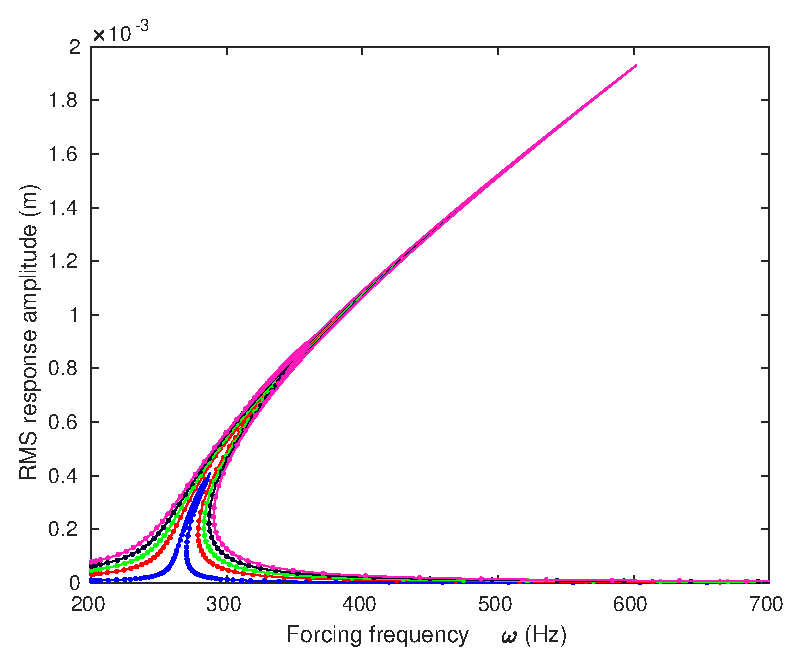
\includegraphics[width=0.7\linewidth]{../../../benchmark1/fig/pnlssfrf_A10_Amp}
        \caption{Amplitude}
      \end{subfigure}%
      \begin{subfigure}{0.5\linewidth}
        \centering
        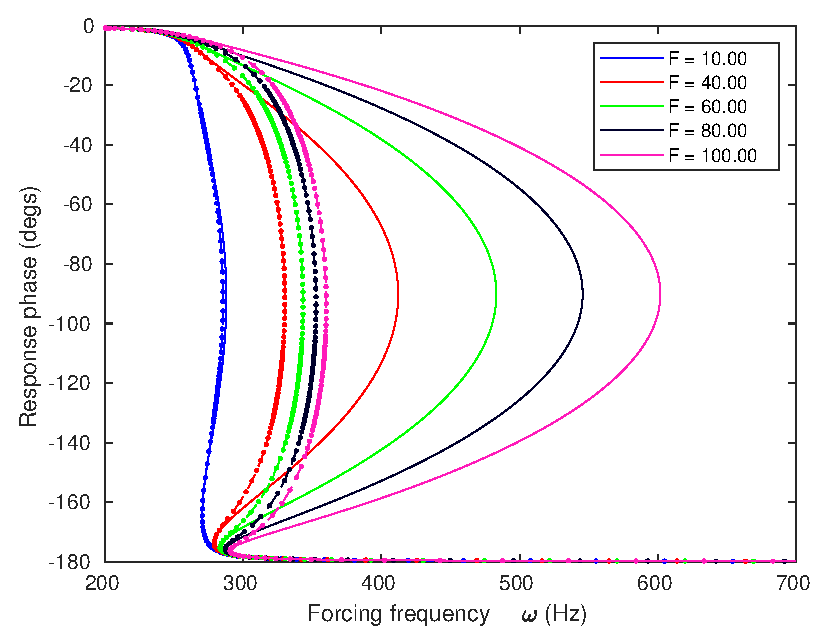
\includegraphics[width=0.7\linewidth]{../../../benchmark1/fig/pnlssfrf_A10_Phase}
        \caption{Phase}
      \end{subfigure}
    \end{figure}
  \end{block}
  \begin{itemize}
  \item The lowest forcing level (F=10) seems to show good matching
  \item For higher levels the matching fails near the peak
  \end{itemize}

  \begin{block}{Multisine (RMS) Excitation Level : 25 N}
    \begin{figure}
      \centering
      \begin{subfigure}{0.5\linewidth}
        \centering
        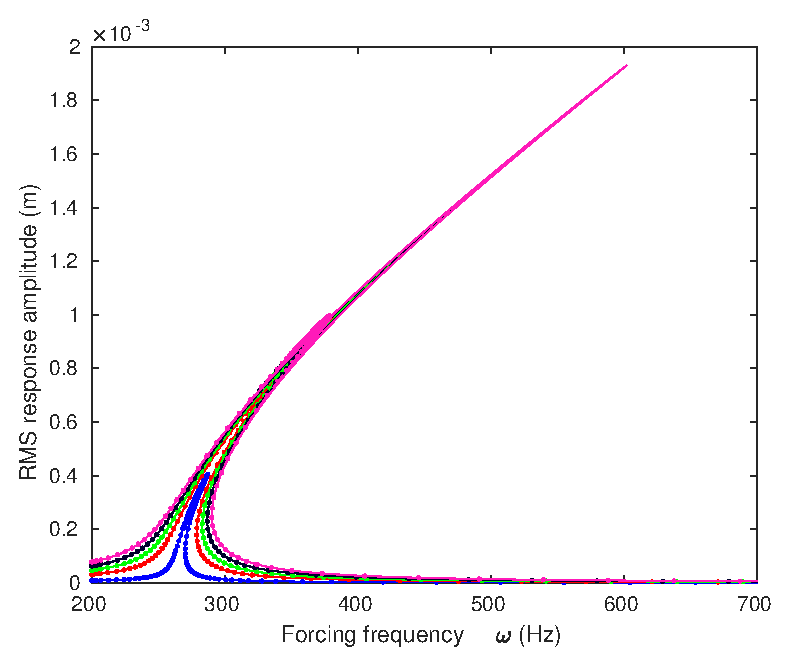
\includegraphics[width=0.8\linewidth]{../../../benchmark1/fig/pnlssfrf_A25_Amp}
        \caption{Amplitude}
      \end{subfigure}%
      \begin{subfigure}{0.5\linewidth}
        \centering
        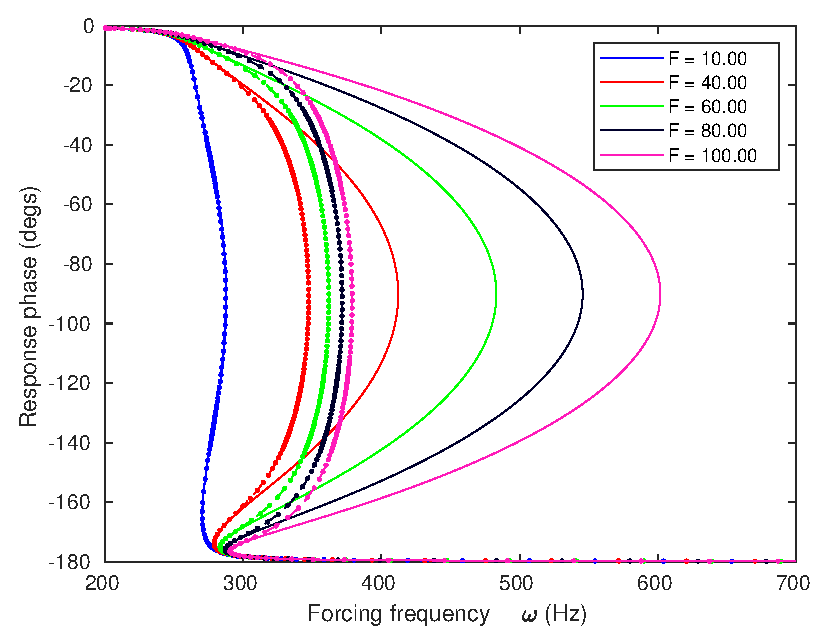
\includegraphics[width=0.8\linewidth]{../../../benchmark1/fig/pnlssfrf_A25_Phase}
        \caption{Phase}
      \end{subfigure}
    \end{figure}
  \end{block}
  \vspace{-0.75cm}  
  \begin{itemize}
  \item The lowest forcing level (F=10) seems to show good matching
    once again
  \item Higher levels match progressively better in the off-peak
    regions than before
  \end{itemize}

  \begin{block}{Multisine (RMS) Excitation Level : 35 N}
    \begin{figure}
      \centering
      \begin{subfigure}{0.5\linewidth}
        \centering
        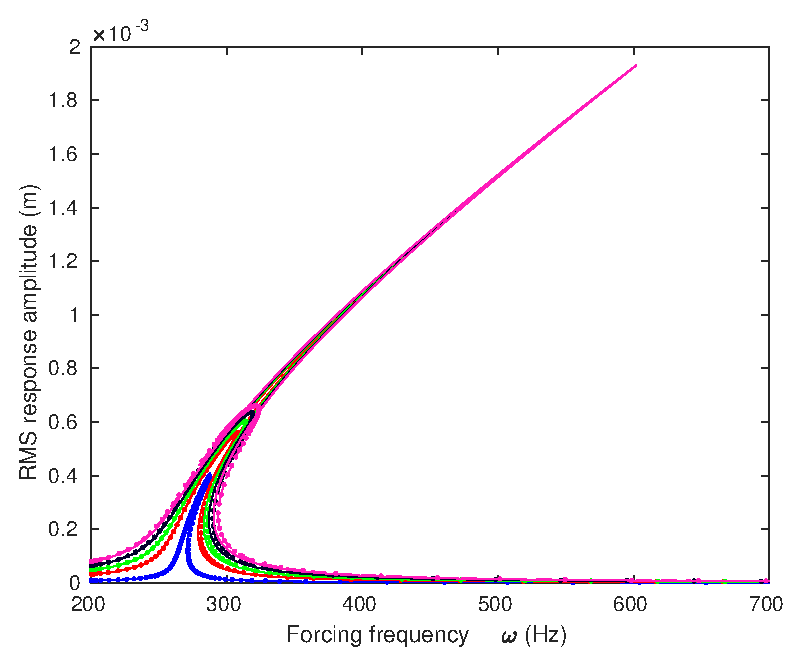
\includegraphics[width=0.8\linewidth]{../../../benchmark1/fig/pnlssfrf_A35_Amp}
        \caption{Amplitude}
      \end{subfigure}%
      \begin{subfigure}{0.5\linewidth}
        \centering
        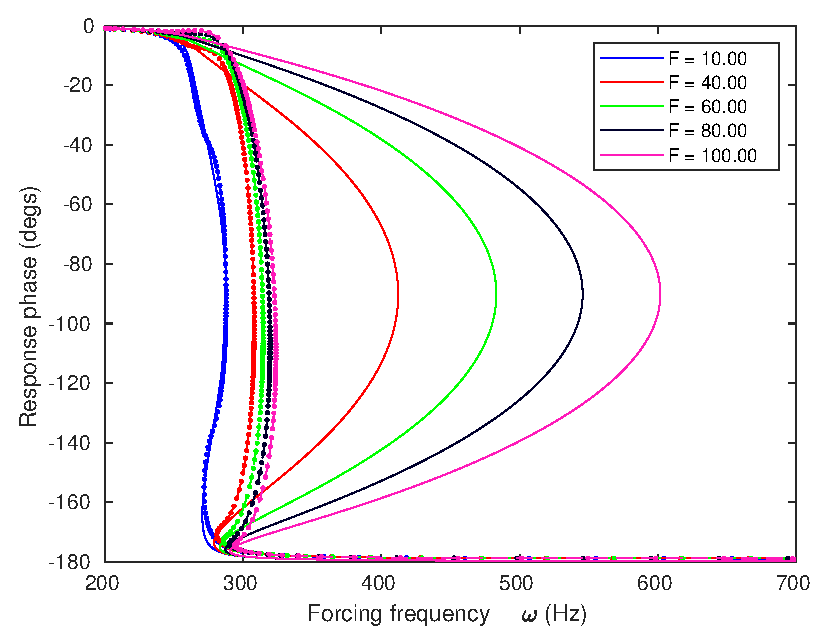
\includegraphics[width=0.8\linewidth]{../../../benchmark1/fig/pnlssfrf_A35_Phase}
        \caption{Phase}
      \end{subfigure}
    \end{figure}
  \end{block}
  \vspace{-0.75cm}  
  \begin{itemize}
  \item The match seems to be worse nearly throughout the response curve
  \end{itemize}  
\end{frame}


\begin{frame}
  \frametitle{Benchmark 4 - Cantilevered Beam with Elastic Dry
    Friction}
  
\end{frame}
\end{document}
%%% Local Variables:
%%% mode: latex
%%% TeX-master: t
%%% End:
